\documentclass{article}
\usepackage[utf8]{inputenc}

% incluir imagens
\usepackage{graphicx}
\graphicspath{ {./images/} }

\title{Construção de Termômetro por um Diodo}
\author{Henrique Poleselo e Rodrigo Canário}
\date{Universidade Federal da Bahia - 2019.1}

\begin{document}

\maketitle

\section{Introdução}
O objetivo deste trabalho é integrar o conhecimento visto na disciplina Dispositivos Eletrônicos sobre diodos, reguladores de tensão e transistores juntamente com Eletrônica Digital para a implementação de circuitos em FPGA.
Usando um diodo semicondutor, seguindo a sua função característica do modelo real, conseguimos relacionar temperatura com os níveis de tensão aplicado ao mesmo. Partindo deste principio conseguimos construir um termomêtro digital.

\section{Embasamento Teórico}
 O fenômeno que exploraremos é devido ao efeito Peltier, que com a aplicação de uma tensão, é criado um gradiente de temperatura que varia juntamente com a corrente. (Fenômeno termoelétrico).
\begin{center}
    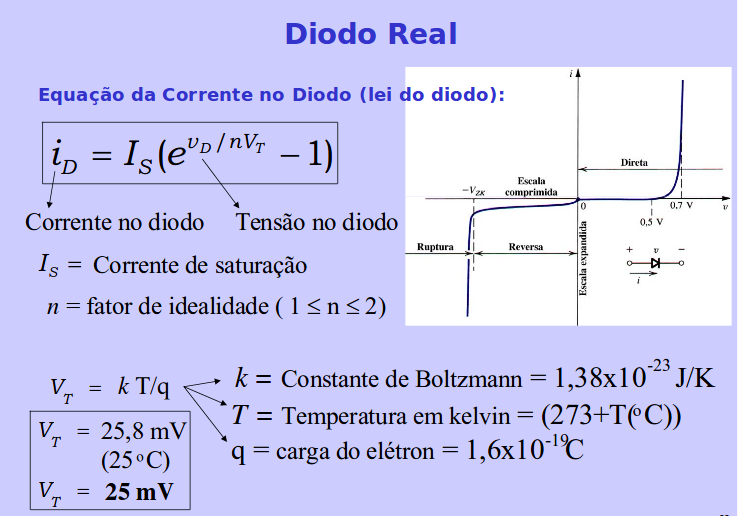
\includegraphics[scale=0.3]{images/img1.png}
    Imagem 1: Modelo do diodo real
\end{center}

\section{Estrutura do projeto}
O trabalho começa no FPGA, onde iremos implementar um algorítmo de Aproximações Sucessivas, i.e um conversor analógico digital. A saída do FPGA (pinos 3.3V) mandando sinais para uma rede R2R

\begin{center}
    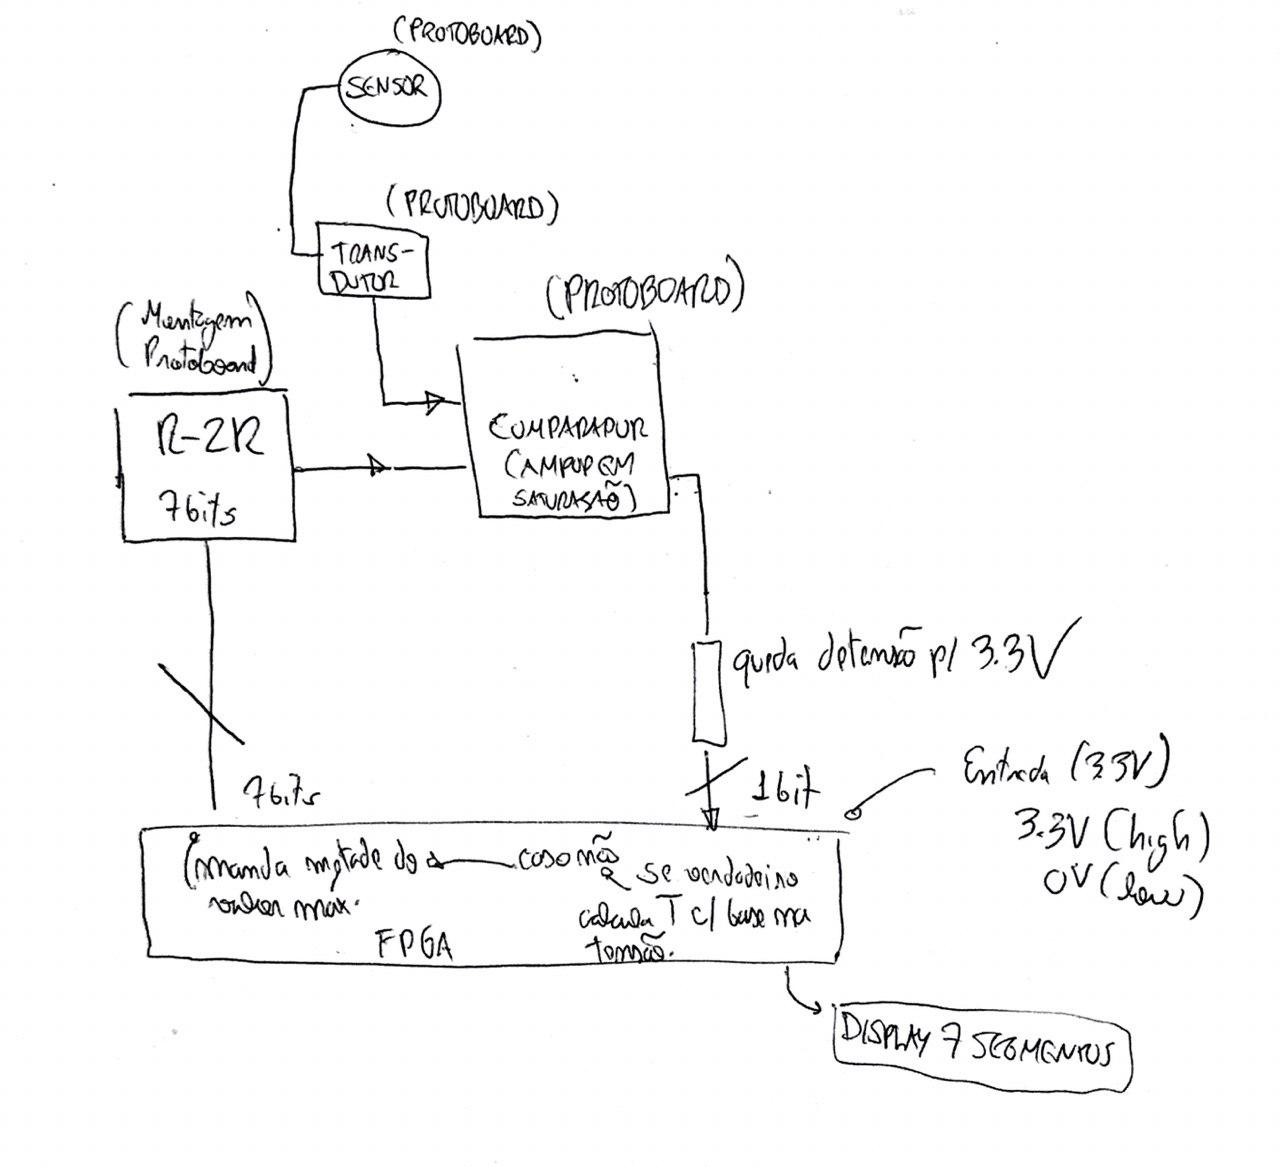
\includegraphics[scale=0.3]{images/sketchprojeto.jpg}
    Imagem 2: Sketch do projeto
\end{center}

\section{Simulação Conversor AD}
Usaremos as redes R-2R, que nos fornecem a possibilidade de conseguir variar níveis de tensão de acordo com as disposições dos resistores, i.e usando uma rede R-2R de 7 bits obteremos: 2(elevado)7 128 valores possiveis pra dividir a tensão de entrada. Como queremos medir de 0 100 graus com passo de 1 grau, então um R-2R de 7 bits será suficiente. Na saída da rede R2R iremos ter um ampop comparador para pegar esses valores de tensão e iremos "filtra-lo". Assim, teremos uma relação tensão-temperatura.

Queremos 12.7V na saída do ampop, começamos alimentando o AMPOP com 12.7V porém a saída, devido à perdas e à todo nosso sistema, possuia sempre aproximadamente -2V do que era inserido. Ou seja, precisávamos aumentar a entrada pra 14.7V de forma que ajustasse a saída do amplificador operacional com 12.7V. Após o encontro com Marcio vimos que de fato é um jargão: se você quer uma saída x de um amplificador operacional, alimente com x + 2V de forma a obter seu x na saída.

% inserir foto da simulacao


\section{Montagem Conversor AD}
Alimentação de tensão simétrica: precisavamos dos +14.7V e -14.7V para a alimentação do Ampop, para isso usamos a fonte de bancada que possui duas saídas de tensão, como mostrado na foto abaixo.
\begin{center}
    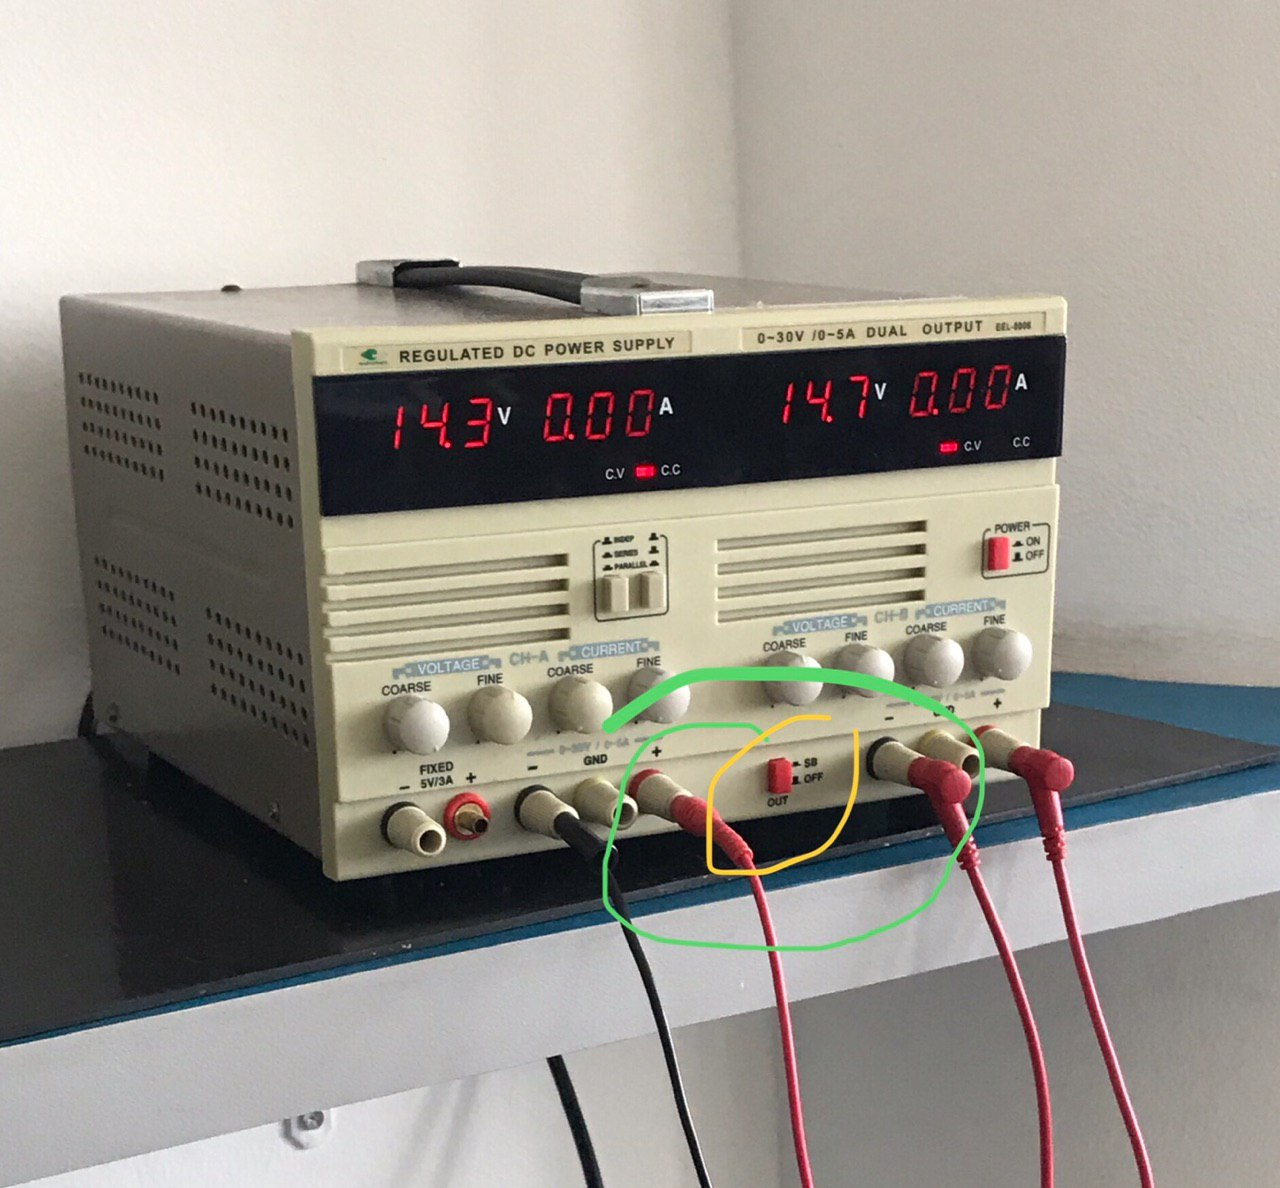
\includegraphics[scale=0.2]{images/fonte.jpeg}
    
    Imagem 2: Fonte de bancada com duas saídas.
\end{center}

Para obter a tensão simétrica precisamos realizar a ligação indicada pelo verde na foto, i.e (+ com -), essa ligação será nosso novo 0. enquanto que o cabo preto na extrema esquerda será nosso menor nível de tensão, que é -15V. Para a configuração ficar correta precisamos apertar o botão vermelho que está circulado em amarelo na imagem acima (ele ativa a ligação interna da fonte pra criar uma fonte simétrica). PS: acabmos errando isso no nosso experimento mas nessa fonte de bancada, elas funcionam sempre como uma "fonte de potência", i.e não adianta só fornecer tensão ao circuito, e sim fornecer o mínimo de corrente também (seguindo a relação $P=VI$) de forma que o circuito em questão seja realmente alimentado.

\begin{center}
    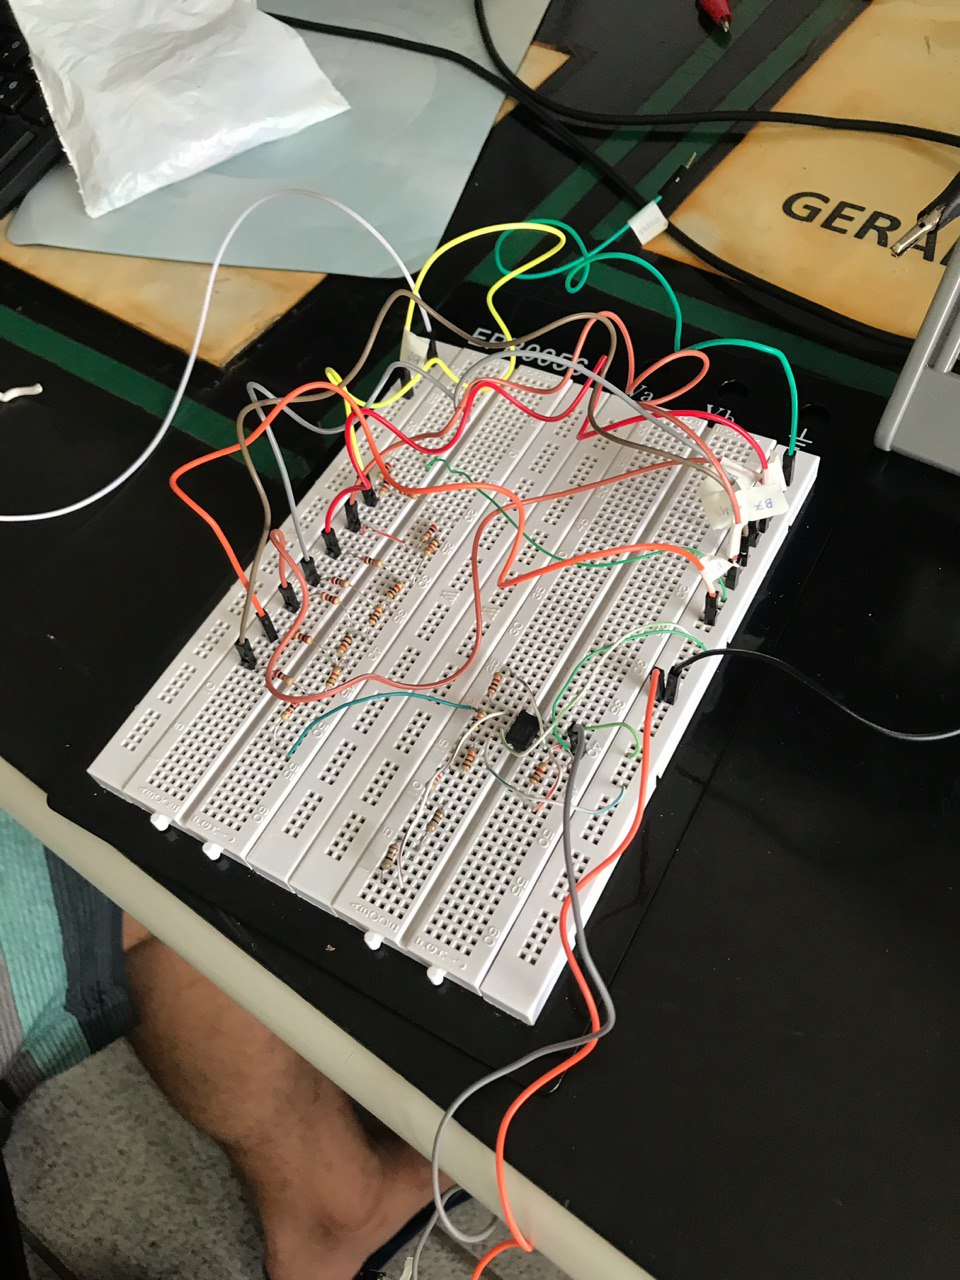
\includegraphics[scale=0.2]{images/montagem_dac.jpeg}
    
    Imagem 3: Montagem do DAC na protoboard.
\end{center}

\section{Caracterização da Curva}
Sabe-se que pra um diodo convencional, a corrente mínima necessária pra sua operação é $20mA$. Como no nosso projeto já há uma tensão alimentando todo o sistema, que é de 12.7V, usaremos a mesma pra alimentar o circuito de sensoriamento, i.e o diodo e o resistor associado para o controle da corrente $Id$. Então, pela lei de Ohm conseguimos determinar qual a resistência necessária: $R=V/I$ $R=12.7/20*10^10-3$

Iremos medir a temperatura usando um termopar, o termopar em questão é um dispositivo que é ligado diretamente ao multímetro e consegue medir a temperatura com uma certa precisão. O termopar em questão foi calibrado pra ser utilizado com o multímetro já mostrado.

\begin{center}
    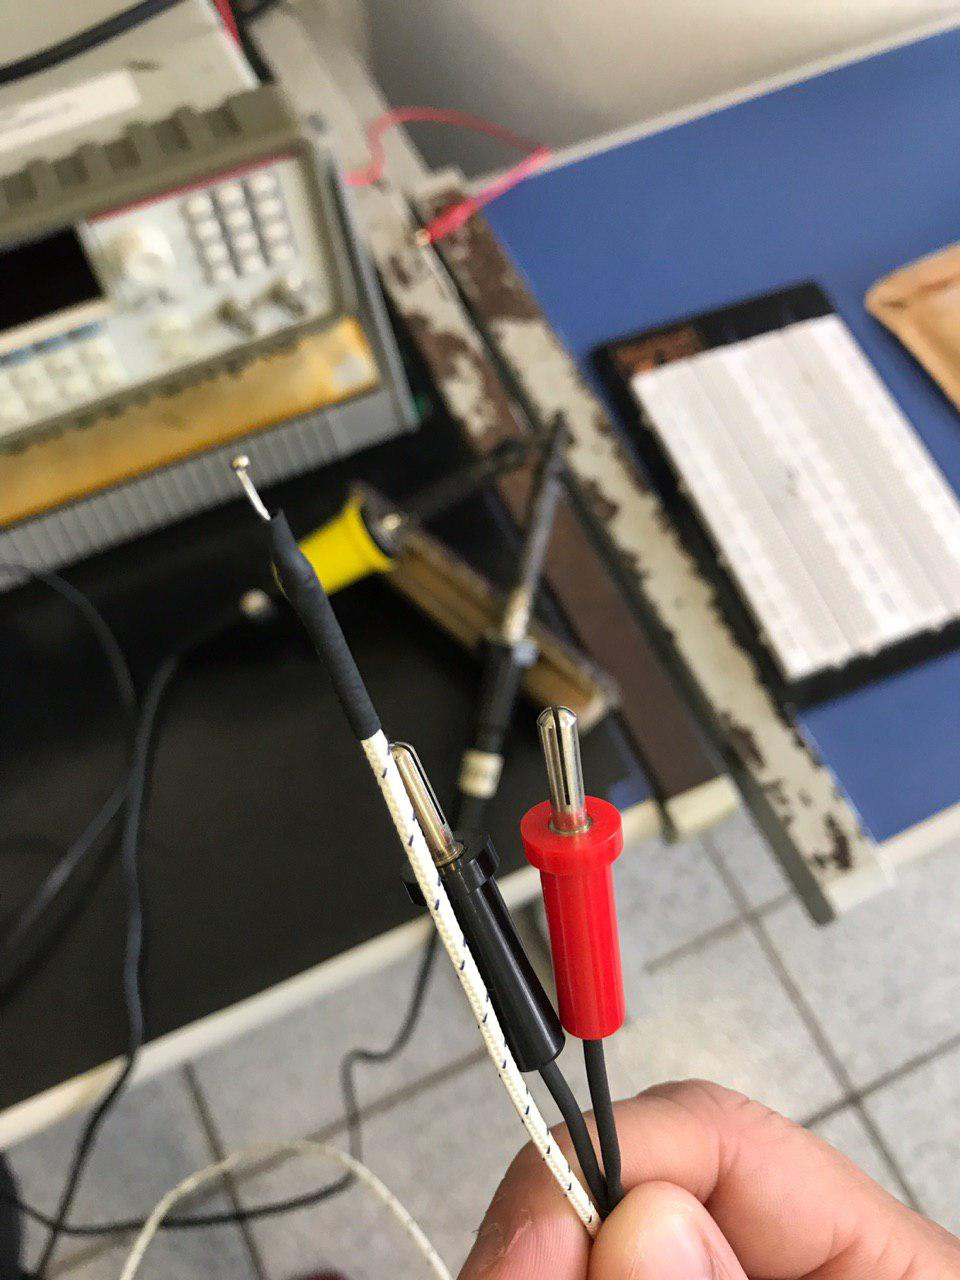
\includegraphics[scale=0.2]{images/termopar.jpg}
    
    Imagem 4: Termopar, note que a ponta em preto possui um contato, este ficará sempre em contato com o diodo para medir a temperatura no diodo.
\end{center}

Colocamos o termopar, usamos um resistor de 680 pois era o que havia disponível, soldamos as pontas do diodo com fios maiores pra facilitar a mobilidade pra medição de temperatura. Como o termopar está junto com o diodo (em toque), movimentamos o diodo e colocamos perto de um ferro de solda, o valor da temperatura aumenta enquanto que o valor da tensão no osciloscópio diminui... isso pois ambos são inversamente proporcionais.
Na prática usamos 680 ohms e 12.4v
Tabela desses valores


\section{Fonte de tensão simétrica}
Para a construção da fonte simétrica

Usamos o modelo de transistor TBJ 2N2219 pois o mesmo consegue suportar até 3W de potência. Segundo o professor, o TBJ que estávamos usando só suportava até 800mW, e pela tensão Vce(coletor-base), resultou em aproximadamente 9V, ou seja, supondo que a corrente que passa na carga é de 0.25A (considerando uma carga de 48 ohms), então a potência dissipada no transistor sera $P=V*I$ $P=0.25*9$ $P=2.22W$

\begin{center}
    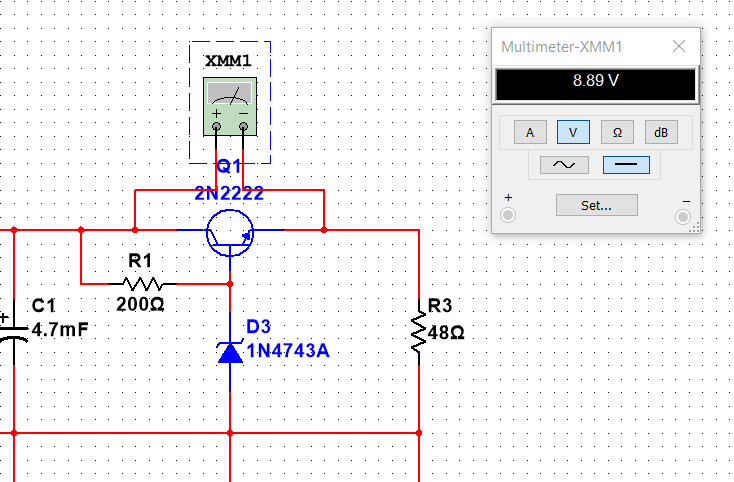
\includegraphics[scale=0.5]{images/potenciatrans.png}
    
    Imagem 5: potência no resistor 48 ohms é $I=V/R$ $I=12.2/48$ $I=0.25A$, ou seja a potência dissipada no resistor será $P=V*I$ $P=12.2*0.25$ ou $P=48*0.25^2$ então $P=3.05W$
\end{center}

Então precisamos de um resistor de potência, que suporte 3W ou mais... assim como um tbj de potência.

\section{Implementação do ADC com VHDL}
O código em VHDL usará uma estrutura de árvore de divisões sucessivas para o "chute" de qual tensão é a presente no diodo, a ávore seguirá a seguinte estrutura:

O chute inicial sendo na metade é mais eficiente pois percorre menos caminho até chegar na tensão que de fato está sendo medida. 

É enviado o sinal para metade da tensão máxima, este então em bits para as 7 portas do FPGA, cada porta tem 3.3V, que será recebido pelo R2R, que irá converter os 7 bits em um valor analógico de tensão, este será uma das entradas do comparador. A outra entrada do comparador é a saída do circuito transdutor (converte o sinal não desejado de tensão para um desejado, i.e condicionado), na faixa em que queremos trabalhar. Assim será comparado no comparador se a tensão enviada pelo FPGA está de acordo com a tensão real no diodo, se sim, uma flag é ativada e calculamos o valor da temperatura no próprio código VHDL segundo a equação que caracterizamos: $v = -1.26*T + 806$
No caso isolamos $T$ e deixamos em função de $v$, pois o que vamos de fato calcular é a temperatura para uma dada tensão (medida). Como sabemos os bits que enviamos para o R2R, então esta será a tensão para o cálculo. Quando calculado o valor será decodificado para BCD e assim enviado para o display os 2 displays de 7 segmentos. 

\end{document}
